% Figure 1 -- Black-Scholes--GJR-GARCH--Sobol research design
% Standalone TikZ source. Compile with: pdflatex article2_research_design_flowchart.tex
% The same code (between \begin{tikzpicture} and \end{tikzpicture}) can be \input into main.tex.
\documentclass[border=2pt]{standalone}
\usepackage[T1]{fontenc}
\usepackage{lmodern}
\usepackage{amsmath}
\usepackage{tikz}
\usetikzlibrary{arrows.meta,positioning,calc,fit,backgrounds}

% ---------- palette (colour-blind safe, prints well in greyscale) ----------
\definecolor{phA}{HTML}{2F5D8A}   % data / sample
\definecolor{phB}{HTML}{2E7D6B}   % volatility model
\definecolor{phC}{HTML}{B7791F}   % option response
\definecolor{phD}{HTML}{8A4F7D}   % sensitivity analysis
\definecolor{ink}{HTML}{1F2933}
\definecolor{mute}{HTML}{52606D}

\begin{document}
\sffamily\hyphenpenalty=10000 \exhyphenpenalty=10000 \tolerance=2000
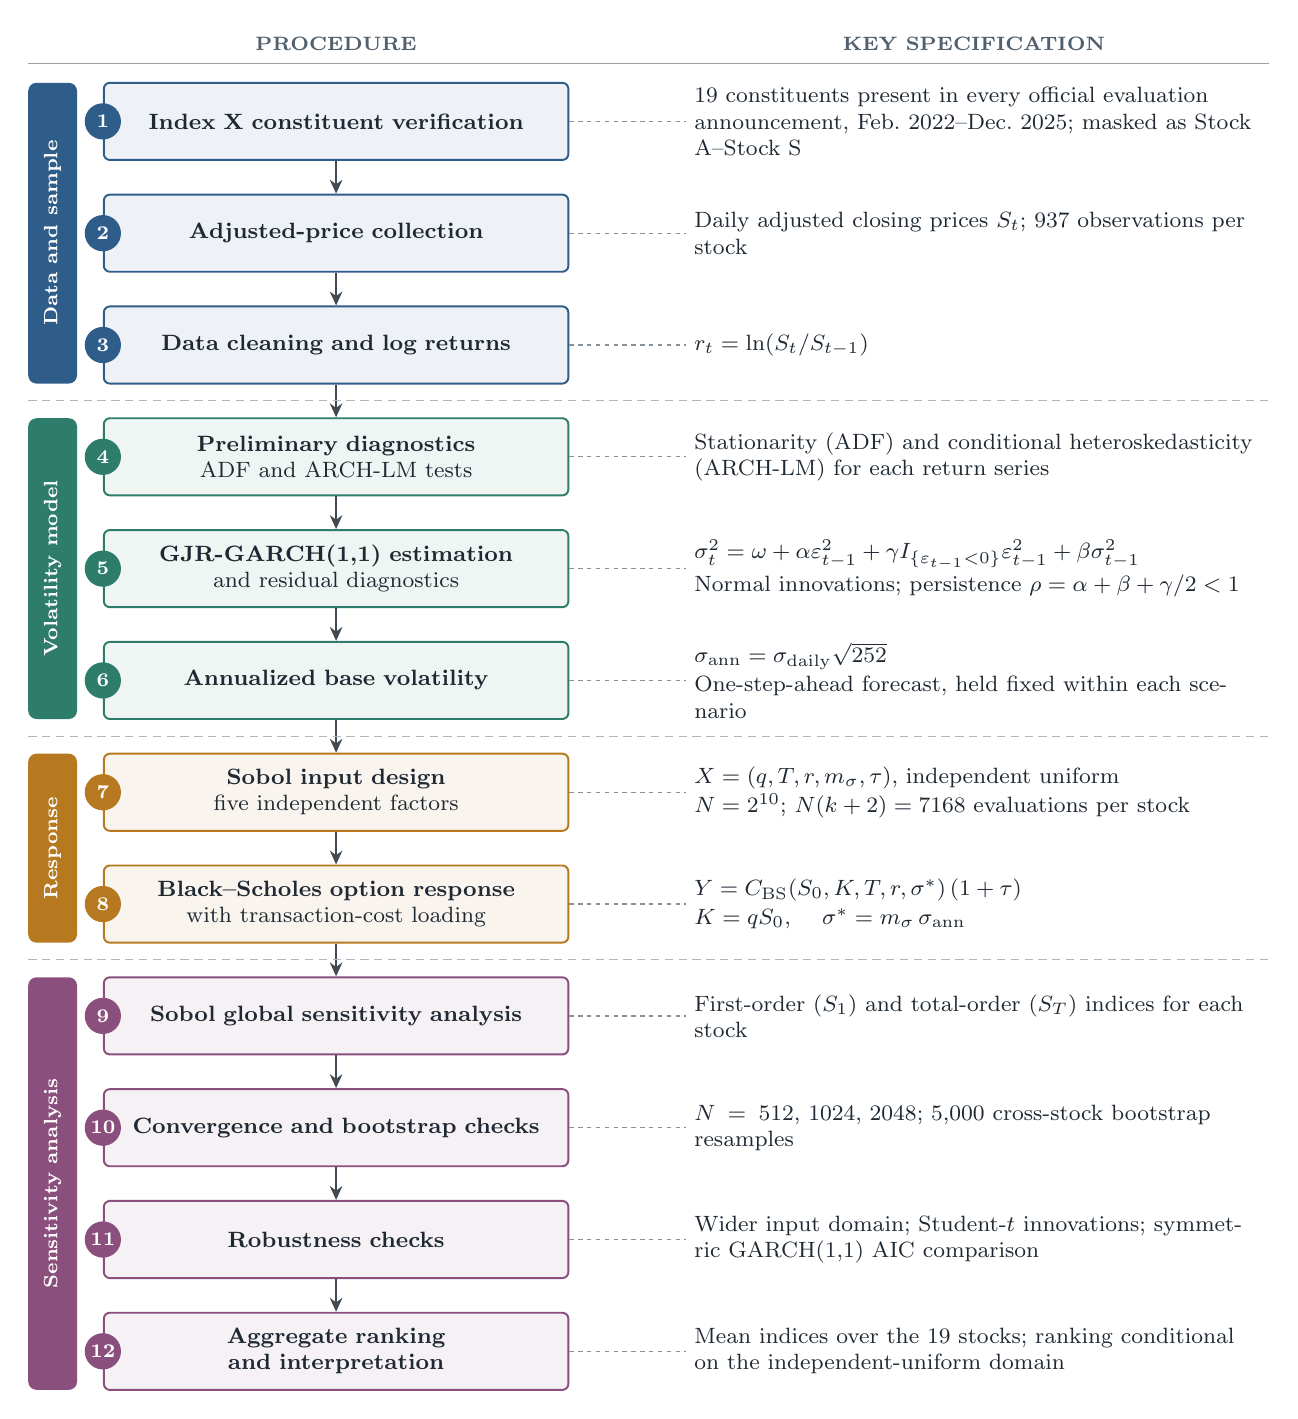
\begin{tikzpicture}[
    font=\footnotesize,
    x=1cm, y=1cm,
    step/.style={rectangle, rounded corners=2.2pt, draw=#1, fill=#1!8, line width=0.7pt,
                 minimum width=5.9cm, minimum height=0.98cm, inner sep=3pt,
                 text=ink, align=center, text width=5.3cm},
    note/.style={rectangle, draw=none, fill=none, minimum width=7.3cm, text width=7.1cm,
                 inner sep=2pt, text=ink, align=left, font=\footnotesize},
    badge/.style={circle, fill=#1, text=white, inner sep=0pt, minimum size=0.46cm,
                  font=\scriptsize\bfseries},
    flow/.style={-{Stealth[length=5pt,width=4.5pt]}, line width=0.8pt, color=ink!85},
    link/.style={line width=0.45pt, color=mute!70, dash pattern=on 1.6pt off 1.6pt},
    phase/.style={rectangle, rounded corners=3pt, fill=#1, text=white, align=center,
                  font=\scriptsize\bfseries, inner sep=0pt, text width=0.62cm}
  ]

% ---------------- geometry ----------------
% column x-positions: phase strip | steps | notes
\def\xs{2.05}      % centre of step column
\def\xn{10.15}      % centre of note column
\def\dy{1.42}      % vertical pitch of steps

% ---------------- steps ----------------
\node[step=phA] (s1) at (\xs, 0*-\dy) {\textbf{Index X constituent verification}};
\node[step=phA] (s2) at (\xs, 1*-\dy) {\textbf{Adjusted-price collection}};
\node[step=phA] (s3) at (\xs, 2*-\dy) {\textbf{Data cleaning and log returns}};

\node[step=phB] (s4) at (\xs, 3*-\dy) {\textbf{Preliminary diagnostics}\\ ADF and ARCH-LM tests};
\node[step=phB] (s5) at (\xs, 4*-\dy) {\textbf{GJR-GARCH(1,1) estimation}\\ and residual diagnostics};
\node[step=phB] (s6) at (\xs, 5*-\dy) {\textbf{Annualized base volatility}};

\node[step=phC] (s7) at (\xs, 6*-\dy) {\textbf{Sobol input design}\\ five independent factors};
\node[step=phC] (s8) at (\xs, 7*-\dy) {\textbf{Black--Scholes option response}\\ with transaction-cost loading};

\node[step=phD] (s9)  at (\xs,  8*-\dy) {\textbf{Sobol global sensitivity analysis}};
\node[step=phD] (s10) at (\xs,  9*-\dy) {\textbf{Convergence and bootstrap checks}};
\node[step=phD] (s11) at (\xs, 10*-\dy) {\textbf{Robustness checks}};
\node[step=phD] (s12) at (\xs, 11*-\dy) {\textbf{Aggregate ranking and interpretation}};

% ---------------- arrows between steps ----------------
\foreach \a/\b in {1/2,2/3,3/4,4/5,5/6,6/7,7/8,8/9,9/10,10/11,11/12}
  \draw[flow] (s\a.south) -- (s\b.north);

% ---------------- step numbers ----------------
\foreach \i/\c in {1/phA,2/phA,3/phA,4/phB,5/phB,6/phB,7/phC,8/phC,9/phD,10/phD,11/phD,12/phD}
  \node[badge=\c] at ($(s\i.west)+(0.0,0.0)$) {\i};

% ---------------- notes (right column) ----------------
\node[note] (n1) at (\xn, 0*-\dy)
  {19 constituents present in every official evaluation announcement, Feb.\ 2022--Dec.\ 2025; masked as Stock A--Stock S};
\node[note] (n2) at (\xn, 1*-\dy)
  {Daily adjusted closing prices $S_t$; 937 observations per stock};
\node[note] (n3) at (\xn, 2*-\dy)
  {$r_t=\ln\!\left(S_t/S_{t-1}\right)$};

\node[note] (n4) at (\xn, 3*-\dy)
  {Stationarity (ADF) and conditional heteroskedasticity (ARCH-LM) for each return series};
\node[note] (n5) at (\xn, 4*-\dy)
  {$\sigma_t^{2}=\omega+\alpha\varepsilon_{t-1}^{2}+\gamma I_{\{\varepsilon_{t-1}<0\}}\varepsilon_{t-1}^{2}+\beta\sigma_{t-1}^{2}$\\[1pt]
   Normal innovations; persistence $\rho=\alpha+\beta+\gamma/2<1$};
\node[note] (n6) at (\xn, 5*-\dy)
  {$\sigma_{\mathrm{ann}}=\sigma_{\mathrm{daily}}\sqrt{252}$\\[1pt]
   One-step-ahead forecast, held fixed within each scenario};

\node[note] (n7) at (\xn, 6*-\dy)
  {$X=(q,T,r,m_\sigma,\tau)$, independent uniform\\[1pt]
   $N=2^{10}$; $N(k+2)=7168$ evaluations per stock};
\node[note] (n8) at (\xn, 7*-\dy)
  {$Y=C_{\mathrm{BS}}(S_0,K,T,r,\sigma^{*})\,(1+\tau)$\\[1pt]
   $K=qS_0$, \quad $\sigma^{*}=m_\sigma\,\sigma_{\mathrm{ann}}$};

\node[note] (n9) at (\xn, 8*-\dy)
  {First-order ($S_1$) and total-order ($S_T$) indices for each stock};
\node[note] (n10) at (\xn, 9*-\dy)
  {$N=512,\,1024,\,2048$; 5{,}000 cross-stock bootstrap resamples};
\node[note] (n11) at (\xn, 10*-\dy)
  {Wider input domain; Student-$t$ innovations; symmetric GARCH(1,1) AIC comparison};
\node[note] (n12) at (\xn, 11*-\dy)
  {Mean indices over the 19 stocks; ranking conditional on the independent-uniform domain};

% ---------------- dashed leaders step -> note ----------------
\foreach \i in {1,...,12}
  \draw[link] (s\i.east) -- (n\i.west |- s\i.east);

% ---------------- phase strips (left) ----------------
\def\pw{0.62}
\def\px{-1.55}
\newcommand{\phasebar}[4]{% colour, first step, last step, label
  \node[phase=#1, minimum height={abs(#3-#2)*\dy cm + 0.98cm}]
    (ph#2) at (\px, {-(#2+#3)/2*\dy}) {\rotatebox{90}{#4}};
}
\phasebar{phA}{0}{2}{Data and sample}
\phasebar{phB}{3}{5}{Volatility model}
\phasebar{phC}{6}{7}{Response}
\phasebar{phD}{8}{11}{Sensitivity analysis}

% ---------------- column headers ----------------
\node[font=\scriptsize\bfseries, text=mute, anchor=south] at (\xs, 0.78) {PROCEDURE};
\node[font=\scriptsize\bfseries, text=mute, anchor=south] at (\xn, 0.78) {KEY SPECIFICATION};
\draw[line width=0.4pt, color=mute!60] (-1.86,0.74) -- (13.9,0.74);

% ---------------- phase separators (thin) ----------------
\foreach \k in {3,6,8}
  \draw[line width=0.35pt, color=mute!45, dash pattern=on 3pt off 2pt]
    (-1.86, {-(\k-0.5)*\dy}) -- (13.9, {-(\k-0.5)*\dy});

\end{tikzpicture}
\end{document}
